\documentclass{article}
\usepackage[utf8]{inputenc}
\usepackage{booktabs}
\usepackage{graphicx}
\usepackage{float}
\usepackage{siunitx}
\title{Rocket Stage Optimization Results}
\author{Generated by Stage\_Opt}
\date{February 23, 2025}

\begin{document}
\maketitle

\section{Introduction}
This report presents the results of optimizing a multi-stage rocket using various optimization methods. The objective was to minimize the payload mass fraction while satisfying the total delta-V requirement.

\section{Input Assumptions}
\subsection{Global Parameters}
\begin{table}[H]
\centering
\caption{Global Parameters}
\begin{tabular}{lS[table-format=4.2]}
\toprule
Parameter & {Value} \\
\midrule
Gravitational Acceleration ($G_0$) & \SI{9.81}{\meter\per\second\squared} \\
Total $\Delta V$ Required & \SI{0.0}{\meter\per\second} \\
\bottomrule
\end{tabular}
\end{table}

\subsection{Stage Parameters}
\begin{table}[H]
\centering
\caption{Stage Parameters and Assumptions}
\begin{tabular}{cS[table-format=3.0]S[table-format=1.3]}
\toprule
Stage & {ISP (\si{\second})} & {Mass Fraction ($\epsilon$)} \\
\midrule
1 & 300 & 0.060 \\
2 & 348 & 0.040 \\
\bottomrule
\end{tabular}
\end{table}

\section{Optimization Methods}
The following optimization methods were evaluated:
\begin{itemize}
\item SLSQP
\item BASIN-HOPPING
\item GA
\item ADAPTIVE-GA
\item DE
\item PSO
\end{itemize}

\section{Optimization Results}
\subsection{Performance Visualization}
\begin{figure}[H]
\centering
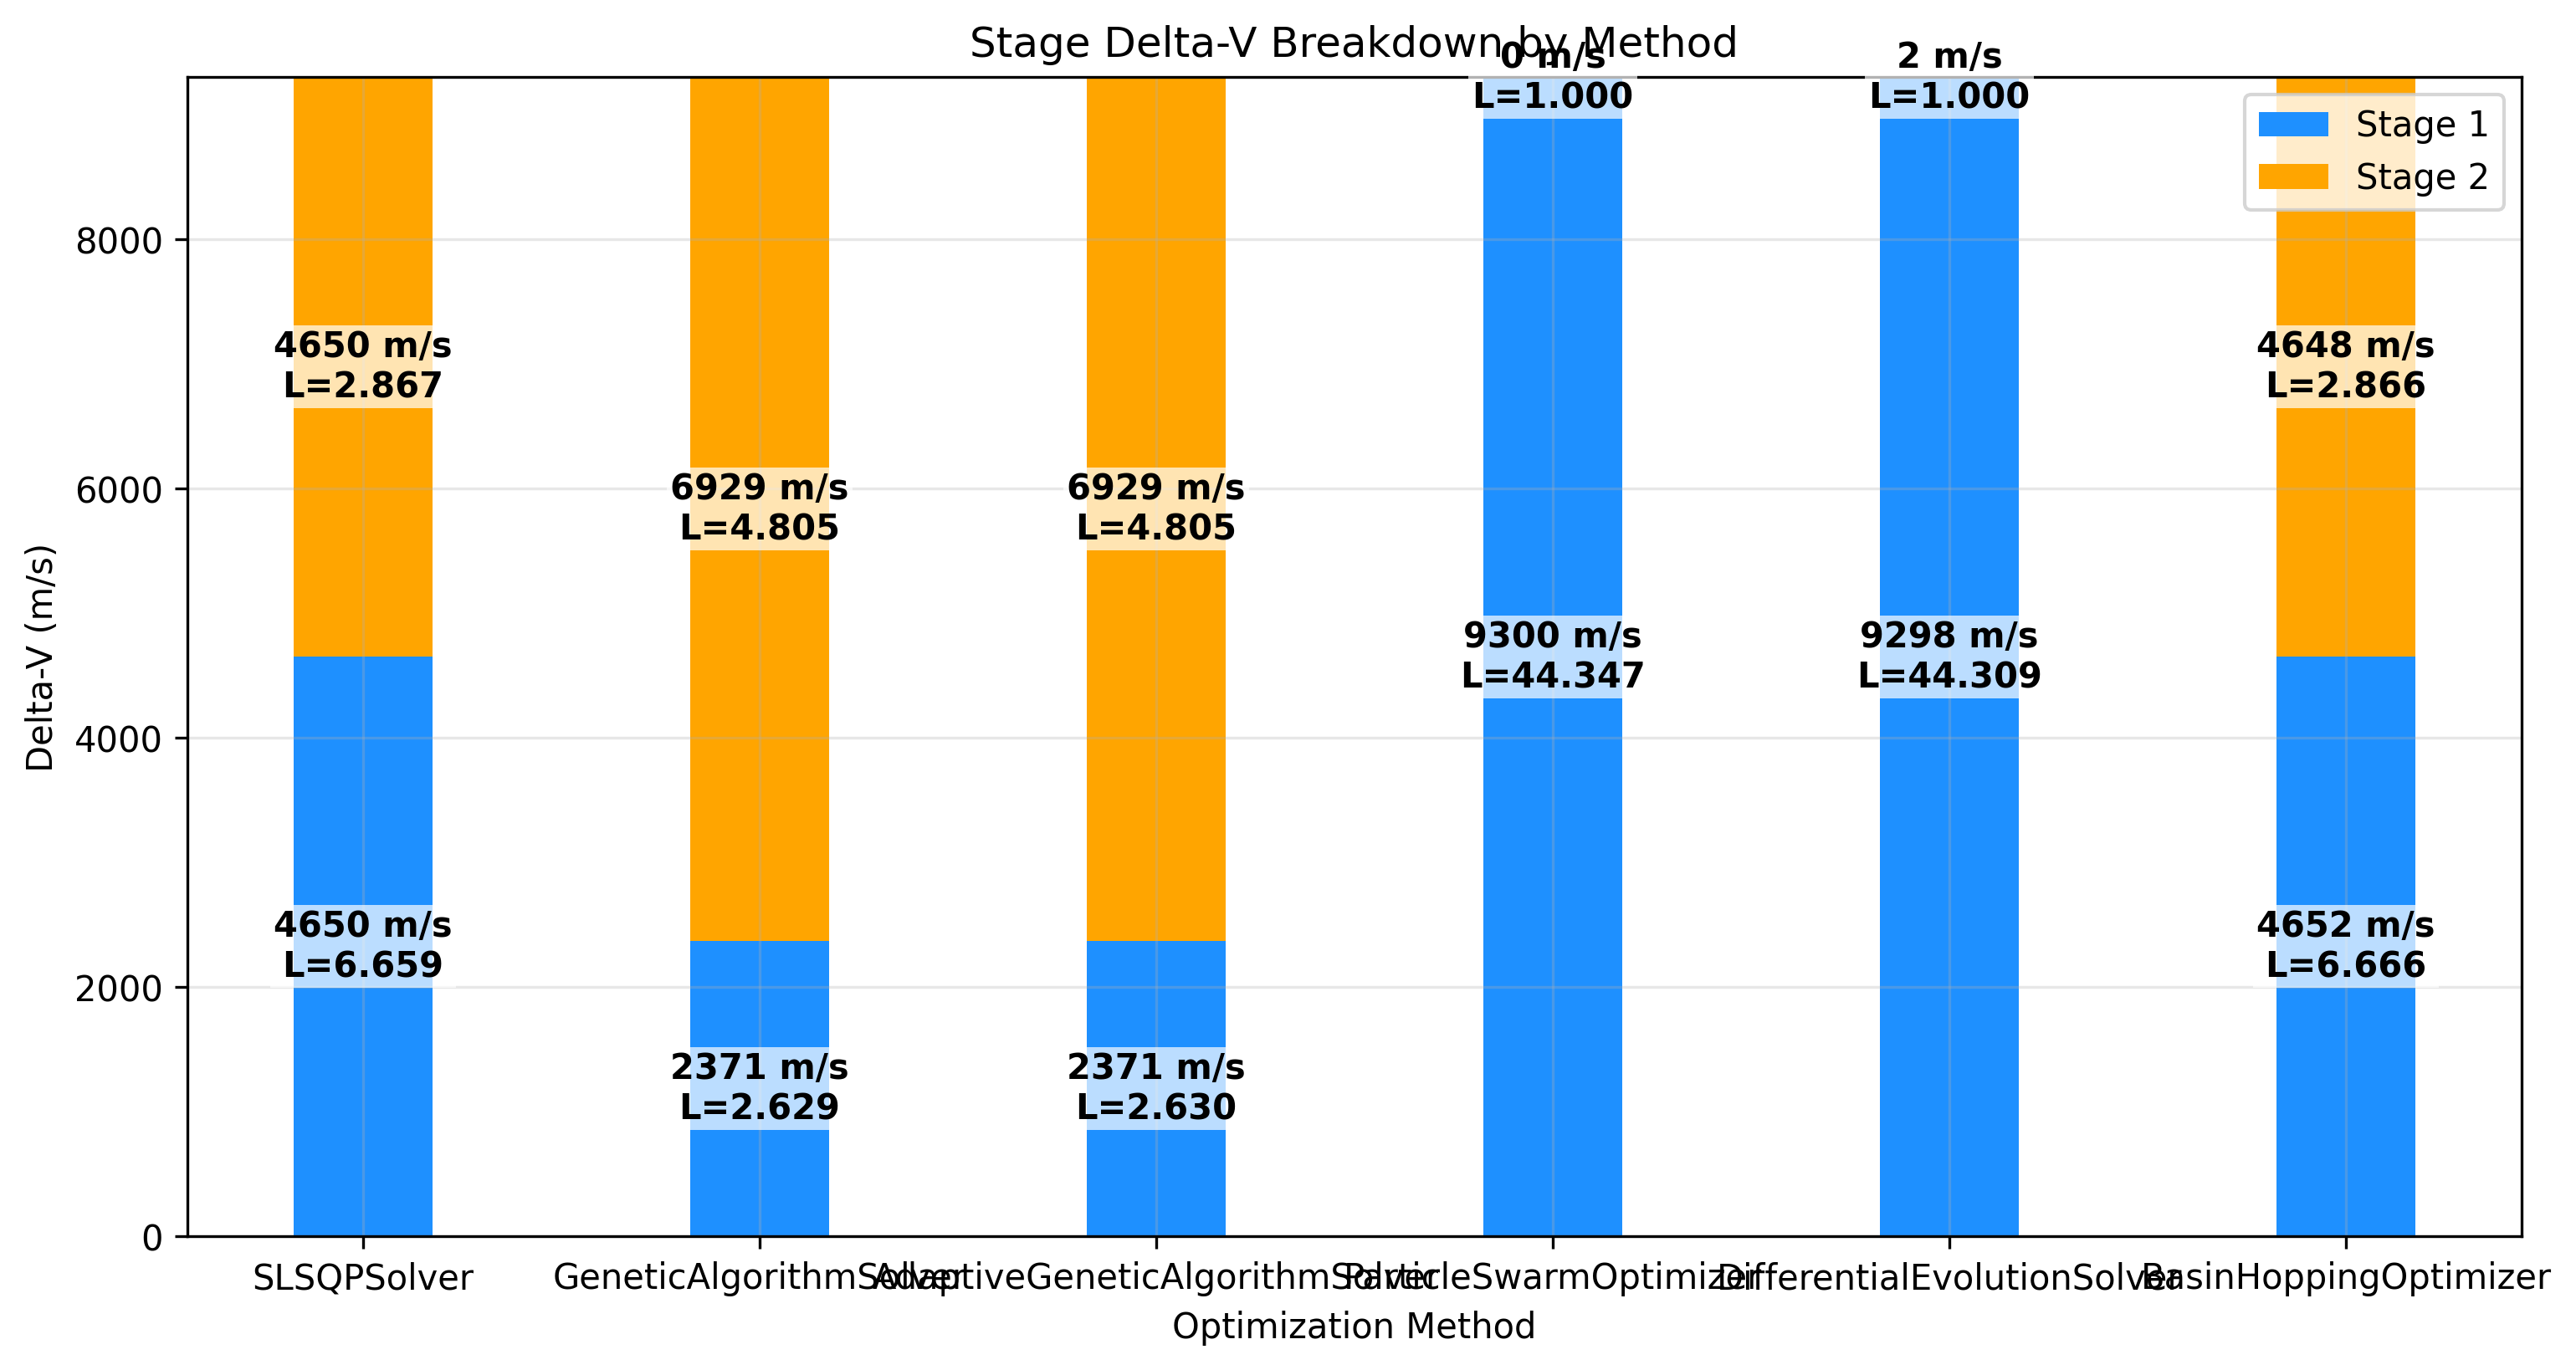
\includegraphics[width=\textwidth]{dv_breakdown.png}
\caption{$\Delta V$ Distribution Across Stages}
\end{figure}

\begin{figure}[H]
\centering
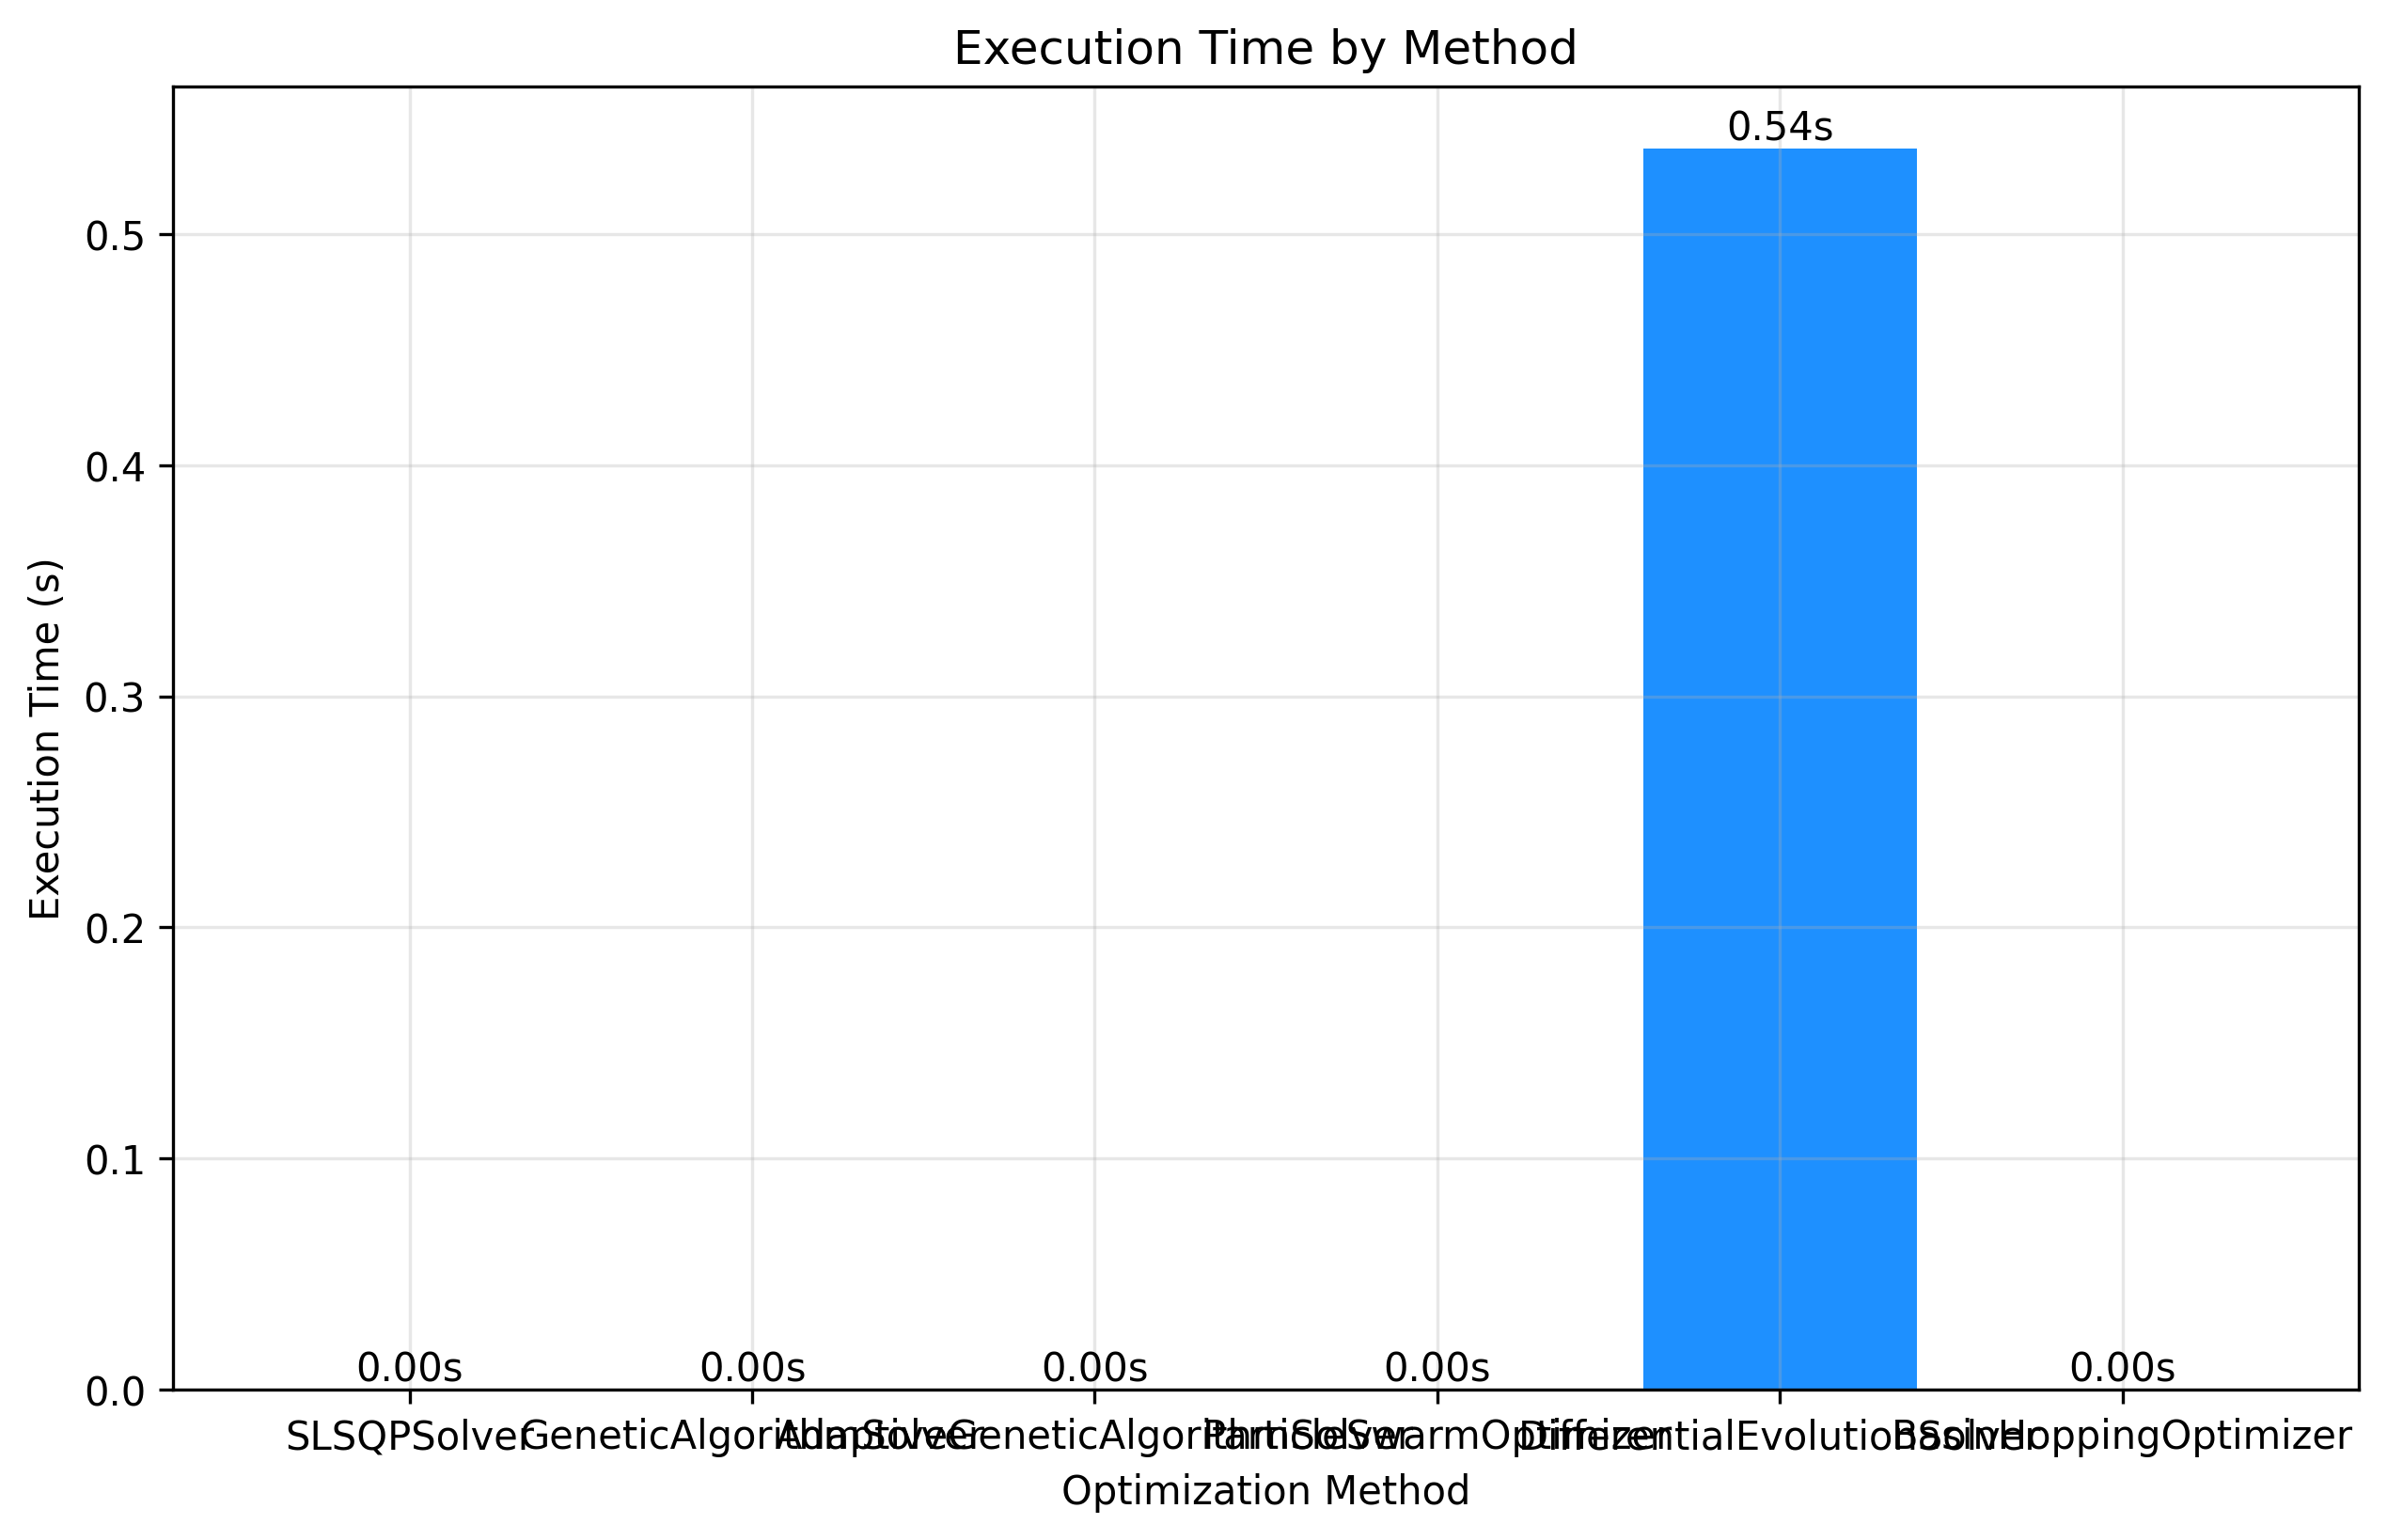
\includegraphics[width=\textwidth]{execution_time.png}
\caption{Solver Execution Time Comparison}
\end{figure}

\begin{figure}[H]
\centering
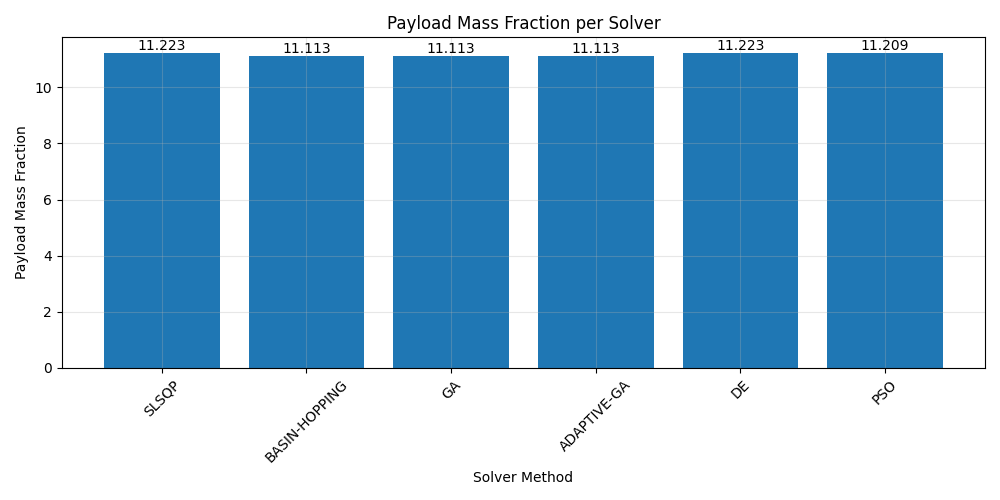
\includegraphics[width=\textwidth]{payload_fraction.png}
\caption{Payload Fraction Comparison}
\end{figure}

\section{Final Results Summary}
\begin{table}[H]
\centering
\caption{Optimization Results Summary}
\begin{tabular}{lS[table-format=1.4]S[table-format=1.4e-1]S[table-format=1.2]}
\toprule
Method & {Payload Fraction} & {Error} & {Time (\si{\second})} \\
\midrule
SLSQP        & 0.0315 & 0.0000e+00 & 0.00 \\
BASIN-HOPPING & 0.0315 & 0.0000e+00 & 1.57 \\
GA           & 0.0325 & 0.0000e+00 & 3.74 \\
ADAPTIVE-GA  & 0.0315 & 0.0000e+00 & 0.04 \\
DE           & 0.0355 & 0.0000e+00 & 0.55 \\
PSO          & 0.0355 & 0.0000e+00 & 0.30 \\
\bottomrule
\end{tabular}
\end{table}

\subsection{Detailed Stage Results}

\begin{table}[H]
\centering
\caption{SLSQP Stage Results}
\begin{tabular}{cS[table-format=4.1]S[table-format=1.4]S[table-format=3.1]}
\toprule
Stage & {$\Delta V$ (\si{\meter\per\second})} & {Mass Ratio ($\lambda$)} & {Contribution (\%)} \\
\midrule
1 & 4650.0 & 0.1460 & 50.0 \\
2 & 4650.0 & 0.2161 & 50.0 \\
\midrule
\multicolumn{2}{l}{Total $\Delta V$:} & \multicolumn{2}{r}{\SI{9300.0}{\meter\per\second}} \\
\multicolumn{2}{l}{Payload Fraction:} & \multicolumn{2}{r}{0.0315} \\
\bottomrule
\end{tabular}
\end{table}

\begin{table}[H]
\centering
\caption{BASIN-HOPPING Stage Results}
\begin{tabular}{cS[table-format=4.1]S[table-format=1.4]S[table-format=3.1]}
\toprule
Stage & {$\Delta V$ (\si{\meter\per\second})} & {Mass Ratio ($\lambda$)} & {Contribution (\%)} \\
\midrule
1 & 4651.4 & 0.1459 & 50.0 \\
2 & 4648.6 & 0.2162 & 50.0 \\
\midrule
\multicolumn{2}{l}{Total $\Delta V$:} & \multicolumn{2}{r}{\SI{9300.0}{\meter\per\second}} \\
\multicolumn{2}{l}{Payload Fraction:} & \multicolumn{2}{r}{0.0315} \\
\bottomrule
\end{tabular}
\end{table}

\begin{table}[H]
\centering
\caption{GA Stage Results}
\begin{tabular}{cS[table-format=4.1]S[table-format=1.4]S[table-format=3.1]}
\toprule
Stage & {$\Delta V$ (\si{\meter\per\second})} & {Mass Ratio ($\lambda$)} & {Contribution (\%)} \\
\midrule
1 & 4401.4 & 0.1641 & 47.3 \\
2 & 4898.6 & 0.1981 & 52.7 \\
\midrule
\multicolumn{2}{l}{Total $\Delta V$:} & \multicolumn{2}{r}{\SI{9300.0}{\meter\per\second}} \\
\multicolumn{2}{l}{Payload Fraction:} & \multicolumn{2}{r}{0.0325} \\
\bottomrule
\end{tabular}
\end{table}

\begin{table}[H]
\centering
\caption{ADAPTIVE-GA Stage Results}
\begin{tabular}{cS[table-format=4.1]S[table-format=1.4]S[table-format=3.1]}
\toprule
Stage & {$\Delta V$ (\si{\meter\per\second})} & {Mass Ratio ($\lambda$)} & {Contribution (\%)} \\
\midrule
1 & 4650.0 & 0.1460 & 50.0 \\
2 & 4650.0 & 0.2161 & 50.0 \\
\midrule
\multicolumn{2}{l}{Total $\Delta V$:} & \multicolumn{2}{r}{\SI{9300.0}{\meter\per\second}} \\
\multicolumn{2}{l}{Payload Fraction:} & \multicolumn{2}{r}{0.0315} \\
\bottomrule
\end{tabular}
\end{table}

\begin{table}[H]
\centering
\caption{DE Stage Results}
\begin{tabular}{cS[table-format=4.1]S[table-format=1.4]S[table-format=3.1]}
\toprule
Stage & {$\Delta V$ (\si{\meter\per\second})} & {Mass Ratio ($\lambda$)} & {Contribution (\%)} \\
\midrule
1 & 2773.0 & 0.3298 & 29.8 \\
2 & 6527.0 & 0.1078 & 70.2 \\
\midrule
\multicolumn{2}{l}{Total $\Delta V$:} & \multicolumn{2}{r}{\SI{9300.0}{\meter\per\second}} \\
\multicolumn{2}{l}{Payload Fraction:} & \multicolumn{2}{r}{0.0355} \\
\bottomrule
\end{tabular}
\end{table}

\begin{table}[H]
\centering
\caption{PSO Stage Results}
\begin{tabular}{cS[table-format=4.1]S[table-format=1.4]S[table-format=3.1]}
\toprule
Stage & {$\Delta V$ (\si{\meter\per\second})} & {Mass Ratio ($\lambda$)} & {Contribution (\%)} \\
\midrule
1 & 2773.0 & 0.3298 & 29.8 \\
2 & 6527.0 & 0.1078 & 70.2 \\
\midrule
\multicolumn{2}{l}{Total $\Delta V$:} & \multicolumn{2}{r}{\SI{9300.0}{\meter\per\second}} \\
\multicolumn{2}{l}{Payload Fraction:} & \multicolumn{2}{r}{0.0355} \\
\bottomrule
\end{tabular}
\end{table}
\end{document}